\chapter{ENFOQUE DE MERCADO.} %(((

\section{Tanque para Aire Comprimido.} % (((
Se realizó el enfoque de mercado que involucra a los siguientes activos.

\subsection{\centering --- Variables ---} % (((
\begin{center}
  \begin{tabular}{|l|l|l|}
    \hline 
    Variable & Descripción   & Unidades\\ \hline 
    Y:  & Precio del activo  & MXN \\ \hline 
    X1: & Edad del activo    & Años \\ \hline 
		X2: & Volumen del activo & \(m ^ 3\) \\ \hline 
  \end{tabular}
\end{center} 
% )))

\subsection{\centering --- Mercado Usado ---} % (((
Se toma la siguiente muestra estadísticamente significativa. \\ 
La comprobación de este hecho se realiza a lo largo de las siguientes secciones.
\begin{center}
	\begin{tabular}{*{4}{|p{2cm}}|}
		\hline 
		MARCA     & EDAD &  VOL   & PRECIO \\ \hline 
		Tankidara & 0    &  1000  & \$61,416.20 \\ \hline 
		Sin Dato  & 39   &  875   & \$19,515.00 \\ \hline 
		Sin Dato  & 11   &  1000  & \$37,729.00 \\ \hline 
		Sin Dato  & 11   &  1000  & \$36,297.90 \\ \hline
	\end{tabular}
\end{center}
% )))

\subsection{\centering --- Matriz de Dispersion ---} % (((
\begin{center}
  \begin{tabular}{|p{11cm}|p{5cm}|}
    \hline
    Gráfica & Interpretación. \\ \hline 
    \begin{minipage}{\textwidth}
    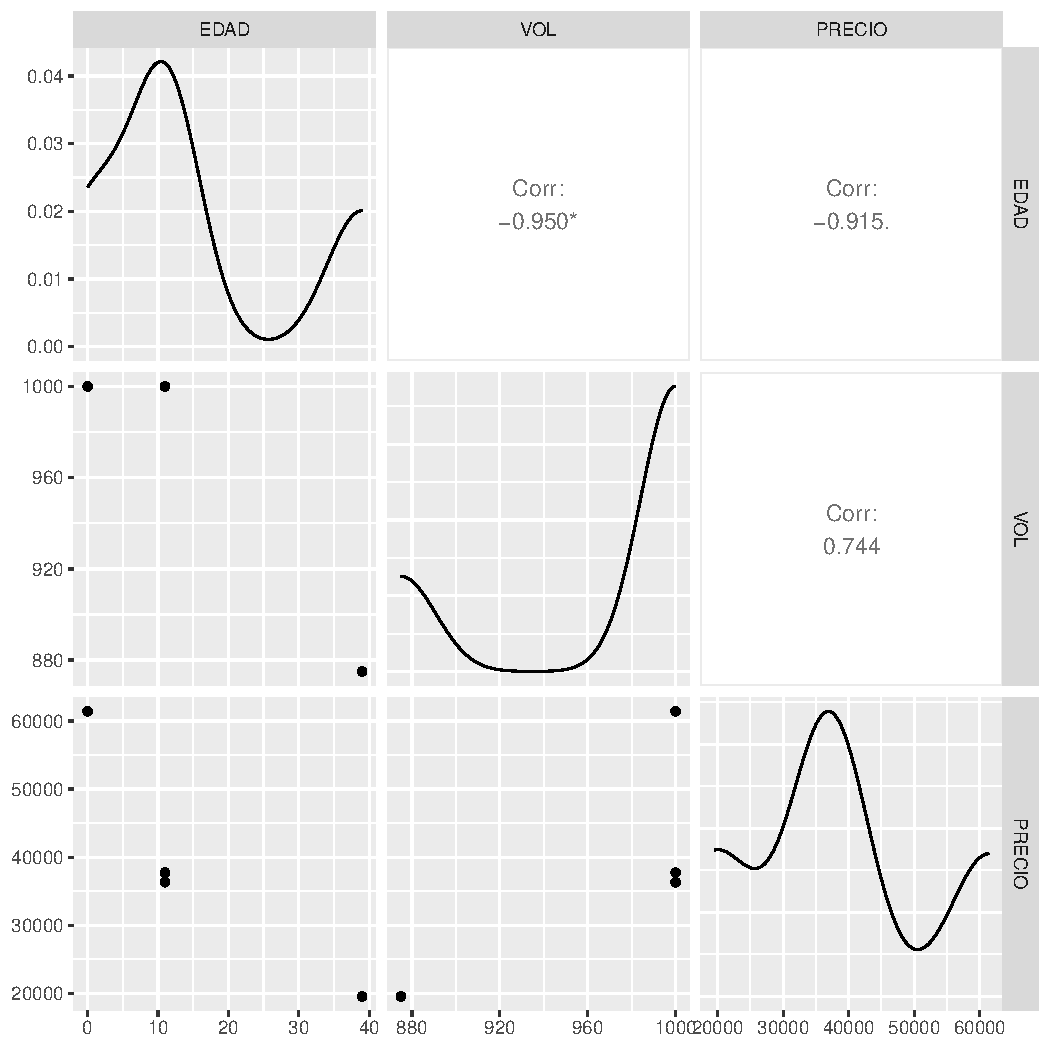
\includegraphics[width= 0.5 \linewidth, page=1]{../0.documentos/3_MERGED_MARKET/1_TANQUE/r/Rplots.pdf}
    \end{minipage} 
    &
		Se tiene una correlación lineal negativa fuerte (el \(91.5\%\) de los datos lo corroboran),
		entre la Edad del Activo, y el Precio del Activo.
		\\ \hline 
  \end{tabular}
\end{center} 
% )))

\subsection{\centering --- Supuestos del Modelo de Regresión ---} % (((

Se realiza el análisis estadístico con un \(90\%\) de confianza. \\ 
Es decir, \(1- \alpha = 0.9\).

\subsubsection{--- Homocedasticidad ---} % (((
\begin{center}
  \begin{tabular}{|l|p{8cm}|}
    \cline{1-2}
    \multicolumn{2}{|c|}{Hipótesis}\\ \cline{1-2}
    \multicolumn{2}{|l|}{\(H_0:\) La varianza de los residuales es constante.} \\ 
    \multicolumn{2}{|l|}{\(H_a:\) La varianza de los residuales no es constante.} \\ \cline{1-2}
    Estadístico de Prueba & \(BP = 4\).\\ \cline{1-2} 
		Región de Rechazo de \(H_0\) & \((0, \alpha )\).\\ \cline{1-2} 
    Valor \(p\) & \(0.1353\).\\ \cline{1-2} 
    Conclusión & Se tiene que \(p> \alpha\). \newline 
		Por tanto no se rechaza \(H_0\). \newline 
		Es decir, la varianza no es constante. \\ \cline{1-2} 
  \end{tabular}
\end{center}
% )))

\subsubsection{--- Independencia ---} % (((
\begin{center}
  \begin{tabular}{|l|p{8cm}|}
    \cline{1-2}
    \multicolumn{2}{|c|}{Hipótesis}\\ \cline{1-2}
    \multicolumn{2}{|l|}{\(H_0:\) Los residuos son independientes.} \\ 
    \multicolumn{2}{|l|}{\(H_a:\) Los residuos no son indpendientes.} \\ \cline{1-2}
    Estadístico de Prueba & \(DW = 2.5\).\\ \cline{1-2} 
		Región de Rechazo de \(H_0\) & \((0, \alpha )\).\\ \cline{1-2} 
    Valor \(p\) & \(1\).\\ \cline{1-2} 
    Conclusión & Se tiene que \(p> \alpha\). \newline 
		Por tanto no se rechaza \(H_0\). \newline 
		Es decir, los residuos son independientes.\\ \cline{1-2} 
  \end{tabular}
\end{center}
% )))

\subsubsection{--- Normalidad ---} % (((
\begin{center}
  \begin{tabular}{|l|p{8cm}|}
    \cline{1-2}
    \multicolumn{2}{|c|}{Hipótesis}\\ \cline{1-2}
    \multicolumn{2}{|l|}{\(H_0:\) Los residuos siguen una distribución normal} \\ 
    \multicolumn{2}{|l|}{\(H_a:\) Los residuos no siguen una distribución normal.} \\ \cline{1-2}
    Estadístico de Prueba & \(W = 0.94466\).\\ \cline{1-2} 
		Región de Rechazo de \(H_0\) & \((0, \alpha )\).\\ \cline{1-2} 
    Valor \(p\) & \(0.683\).\\ \cline{1-2} 
    Conclusión & Se tiene que \(p> \alpha\). \newline 
		Por tanto no se rechaza \(H_0\). \newline 
		Es decir, los residuos siguen una distribución normal.\\ \cline{1-2} 
  \end{tabular}
\end{center}
% )))

% )))

\subsection{\centering Modelo de Regresión Estimado ---} % (((
\begin{align}
	Y & = &  418357.3  & -2218.4 \cdot X_1     & -356.9 \cdot X_2   \\[2mm]
	\mbox{Precio} & = &  418,357.3 & - 2,218.4 \cdot (\mbox{Edad}) & - 358.9 \cdot (\mbox{Volumen})
	\label{eq:1}
\end{align}
% )))

\subsection{\centering --- Tabla Anova ---} % (((
\begin{center}
  \begin{tabular}{|l|l|l|l|l|}
    \hline 
    Fuentes de Variación  & Suma de Cuadrados & Grados de Libertad & Cuadrados Medios & F\\ \hline 
    Regresión           & 889772620 &           \(2\) & 444886310 & \(434.4493\) \\ \hline 
    Error               &   1024024 &          \(1\)  &   1024024 &   \\ \hline 
    Totales             & 890796644 &          \(3\)  & 445910334 &   \\ \hline 
  \end{tabular}
\end{center} 
% )))

\subsection{\centering --- Prueba de Significancia del Modelo ---} % (((
Se comprueba la significancia del modelo con el estadístico \(F\) de la Tabla Anova.
\begin{center}
  \begin{tabular}{|l|p{6cm}|}
    \cline{1-2}
    \multicolumn{2}{|c|}{Hipótesis}\\ \cline{1-2}
    \multicolumn{2}{|l|}{\(H_0:\) El modelo no es significativo.} \\ 
    \multicolumn{2}{|l|}{\(H_a:\) El modelo es significativo.} \\ \cline{1-2}
    Estadístico de Prueba & \(434.4493\).\\ \cline{1-2} 
		Región de Rechazo de \(H_0\) & \((0, \alpha )\).\\ \cline{1-2} 
    Valor \(p\) & \(0.03391\).\\ \cline{1-2} 
    Conclusión & Se tiene que \(p<\alpha\). \newline 
		Por tanto se rechaza \(H_0\). \newline 
		Es decir, el modelo es significativo.\\ \cline{1-2} 
  \end{tabular}
\end{center} 
% )))

\subsection{\centering Estimación del Valor de Mercado aplicado al Activo.} % (((
Se obtiene el valor de mercado por medio de las características del activo y el modelo de regresión \eqref{eq:1}.
\begin{center}
  \begin{tabular}{|l|l|l|}
    \hline 
		Descripción   & Unidades  & Activo \\ \hline 
    Edad del activo    & Años      & 2      \\ \hline 
		Volumen del activo & \(m ^ 3\) & 1000   \\ \hline 
		Precio del activo   & MXN       & \$53,845.47 \\ \hline 
  \end{tabular}
\end{center} 
% )))

% )))

\section{Polipasto Eléctrico.} % (((
Se realizó el enfoque de mercado que involucra a los siguientes activos.

\subsection{\centering --- Variables ---} % (((
\begin{center}
  \begin{tabular}{|l|l|l|}
    \hline 
    Variable & Descripción   & Unidades\\ \hline 
    Y:  & Precio del activo  & MXN \\ \hline 
    X1: & Edad del activo    & Años \\ \hline 
		X2: & Toneladas de cap.  & \(1000kg\) \\ \hline 
  \end{tabular}
\end{center} 
% )))

\subsection{\centering --- Mercado Usado ---} % (((
Se toma la siguiente muestra estadísticamente significativa. \\ 
La comprobación de este hecho se realiza a lo largo de las siguientes secciones.
\begin{center}
	\begin{tabular}{*{4}{|p{2cm}}|}
		\hline 
MARCA &     EDAD&   TON & PRECIO \\ \hline 
P\&GM &    0  &  3   & \$62,287.50 \\ \hline
2    &    7  &  1.6  & \$33,836.50 \\ \hline
3    &    25 &  1    & \$48,026.00 \\ \hline
5    &    11 &  1.6  & \$40,385.50 \\ \hline
	\end{tabular}
\end{center}
% )))

\subsection{\centering --- Matriz de Dispersion ---} % (((
\begin{center}
  \begin{tabular}{|p{11cm}|p{5cm}|}
    \hline
    Gráfica & Interpretación. \\ \hline 
    \begin{minipage}{\textwidth}
    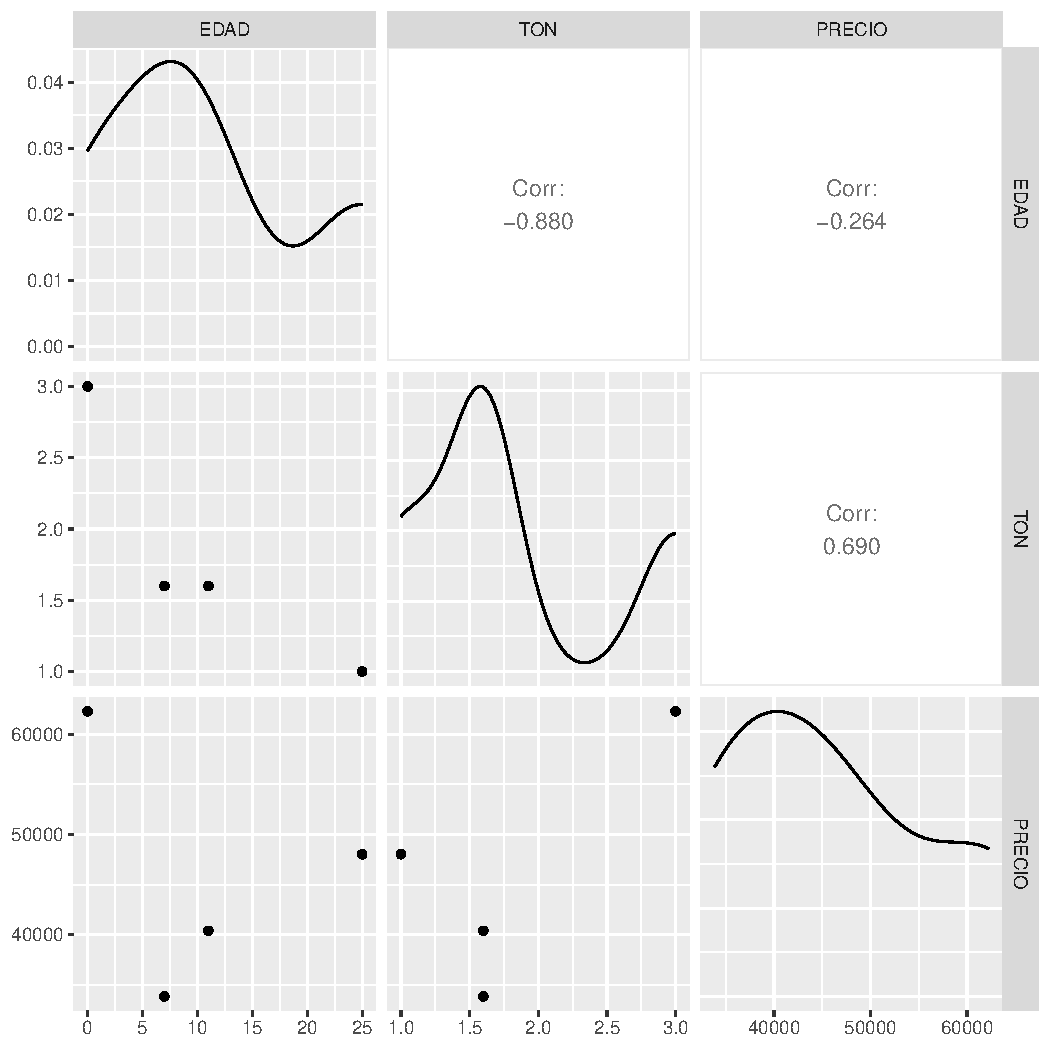
\includegraphics[width= 0.5 \linewidth, page=1]{../0.documentos/3_MERGED_MARKET/2_POLIPASTO/r/Rplots.pdf}
    \end{minipage} 
    &
		Se tiene una correlación lineal negativa fuerte (el \(88.0\%\) de los datos lo corroboran),
		entre las Toneladas de Cap. del Activo, y el Precio del Activo.
		\\ \hline 
  \end{tabular}
\end{center} 
% )))

\subsection{\centering --- Supuestos del Modelo de Regresión ---} % (((

Se realiza el análisis estadístico con un \(90\%\) de confianza. \\ 
Es decir, \(1- \alpha = 0.9\).

\subsubsection{--- Homocedasticidad ---} % (((
\begin{center}
  \begin{tabular}{|l|p{8cm}|}
    \cline{1-2}
    \multicolumn{2}{|c|}{Hipótesis}\\ \cline{1-2}
    \multicolumn{2}{|l|}{\(H_0:\) La varianza de los residuales es constante.} \\ 
    \multicolumn{2}{|l|}{\(H_a:\) La varianza de los residuales no es constante.} \\ \cline{1-2}
    Estadístico de Prueba & \(BP = 1.5527\).\\ \cline{1-2} 
		Región de Rechazo de \(H_0\) & \((0, \alpha )\).\\ \cline{1-2} 
    Valor \(p\) & \(0.4601\).\\ \cline{1-2} 
    Conclusión & Se tiene que \(p> \alpha\). \newline 
		Por tanto no se rechaza \(H_0\). \newline 
		Es decir, la varianza no es constante. \\ \cline{1-2} 
  \end{tabular}
\end{center}
% )))

\subsubsection{--- Independencia ---} % (((
\begin{center}
  \begin{tabular}{|l|p{8cm}|}
    \cline{1-2}
    \multicolumn{2}{|c|}{Hipótesis}\\ \cline{1-2}
    \multicolumn{2}{|l|}{\(H_0:\) Los residuos son independientes.} \\ 
    \multicolumn{2}{|l|}{\(H_a:\) Los residuos no son indpendientes.} \\ \cline{1-2}
    Estadístico de Prueba & \(DW = 1.3517\).\\ \cline{1-2} 
		Región de Rechazo de \(H_0\) & \((0, \alpha )\).\\ \cline{1-2} 
    Valor \(p\) & \(1\).\\ \cline{1-2} 
    Conclusión & Se tiene que \(p> \alpha\). \newline 
		Por tanto no se rechaza \(H_0\). \newline 
		Es decir, los residuos son independientes.\\ \cline{1-2} 
  \end{tabular}
\end{center}
% )))

\subsubsection{--- Normalidad ---} % (((
\begin{center}
  \begin{tabular}{|l|p{8cm}|}
    \cline{1-2}
    \multicolumn{2}{|c|}{Hipótesis}\\ \cline{1-2}
    \multicolumn{2}{|l|}{\(H_0:\) Los residuos siguen una distribución normal} \\ 
    \multicolumn{2}{|l|}{\(H_a:\) Los residuos no siguen una distribución normal.} \\ \cline{1-2}
    Estadístico de Prueba & \(W = 0.88264\).\\ \cline{1-2} 
		Región de Rechazo de \(H_0\) & \((0, \alpha )\).\\ \cline{1-2} 
    Valor \(p\) & \(0.35\).\\ \cline{1-2} 
    Conclusión & Se tiene que \(p> \alpha\). \newline 
		Por tanto no se rechaza \(H_0\). \newline 
		Es decir, los residuos siguen una distribución normal.\\ \cline{1-2} 
  \end{tabular}
\end{center}
% )))

% )))

\subsection{\centering Modelo de Regresión Estimado ---} % (((
\begin{align}
	Y & = &              -25,647 & + 1,771 \cdot X_1           & + 29,299   \cdot X_2   \\[2mm]
	\mbox{Precio} & = &  -25,647 & + 1,771 \cdot (\mbox{Edad}) & + 29,299   \cdot (\mbox{Ton})
	\label{eq:2}
\end{align}
% )))

\subsection{\centering --- Tabla Anova ---} % (((
\begin{center}
  \begin{tabular}{|l|l|l|l|l|}
    \hline 
    Fuentes de Variación  & Suma de Cuadrados & Grados de Libertad & Cuadrados Medios & F\\ \hline 
Regresión  &  448627750.2         &  2     & 224313875.1 &1391.228 \\ \hline
Error      &     161234.5         &  1     &    161234.5 &  \\ \hline
Totales    &  448788984.7         &  3     & 224475109.6 &  \\ \hline
  \end{tabular}
\end{center} 
% )))

\subsection{\centering --- Prueba de Significancia del Modelo ---} % (((
Se comprueba la significancia del modelo con el estadístico \(F\) de la Tabla Anova.
\begin{center}
  \begin{tabular}{|l|p{6cm}|}
    \cline{1-2}
    \multicolumn{2}{|c|}{Hipótesis}\\ \cline{1-2}
    \multicolumn{2}{|l|}{\(H_0:\) El modelo no es significativo.} \\ 
    \multicolumn{2}{|l|}{\(H_a:\) El modelo es significativo.} \\ \cline{1-2}
    Estadístico de Prueba & \(1391.228\).\\ \cline{1-2} 
		Región de Rechazo de \(H_0\) & \((0, \alpha )\).\\ \cline{1-2} 
    Valor \(p\) & \(0.01895\).\\ \cline{1-2} 
    Conclusión & Se tiene que \(p<\alpha\). \newline 
		Por tanto se rechaza \(H_0\). \newline 
		Es decir, el modelo es significativo.\\ \cline{1-2} 
  \end{tabular}
\end{center} 
% )))

\subsection{\centering Estimación del Valor de Mercado aplicado al Activo.} % (((
Se obtiene el valor de mercado por medio de las características del activo y el modelo de regresión \eqref{eq:2}.
\begin{center}
  \begin{tabular}{|l|l|l|}
    \hline 
		Descripción   & Unidades  & Activo \\ \hline 
    Edad del activo    & Años      & 2      \\ \hline 
		Toneladas de cap.  & \(1000kg\) & 2   \\ \hline 
		Precio del activo   & MXN       & \$30,070.81  \\ \hline 
  \end{tabular}
\end{center} 
% )))

% )))

\section{Bombo Batidor/Mezclador para Cofitería.} % (((
Se realizó el enfoque de mercado que involucra a los siguientes activos.

\subsection{\centering --- Variables ---} % (((
\begin{center}
  \begin{tabular}{|l|l|l|}
    \hline 
    Variable & Descripción   & Unidades\\ \hline 
    Y:  & Precio del activo  & MXN \\ \hline 
    X1: & Edad del activo    & Años \\ \hline 
		X2: & Volumen  & \(m ^ 3\) \\ \hline 
  \end{tabular}
\end{center} 
% )))

\subsection{\centering --- Mercado Usado ---} % (((
Se toma la siguiente muestra estadísticamente significativa. \\ 
La comprobación de este hecho se realiza a lo largo de las siguientes secciones.
\begin{center}
	\begin{tabular}{*{4}{|p{2cm}}|}
		\hline 
MARCA    & EDAD  & VOL  & PRECIO \\ \hline
COMFIT   & 0     & 2.7  & \$38,9971.12 \\ \hline
Sin Dato & 0     & 2.7  & \$36,6545.35 \\ \hline
CBA4     & 50    & 2.7  & \$14,0803.50 \\ \hline
CP4      & 34    & 3.2  & \$21,8300.00 \\ \hline
	\end{tabular}
\end{center}
% )))

\subsection{\centering --- Matriz de Dispersion ---} % (((
\begin{center}
  \begin{tabular}{|p{11cm}|p{5cm}|}
    \hline
    Gráfica & Interpretación. \\ \hline 
    \begin{minipage}{\textwidth}
    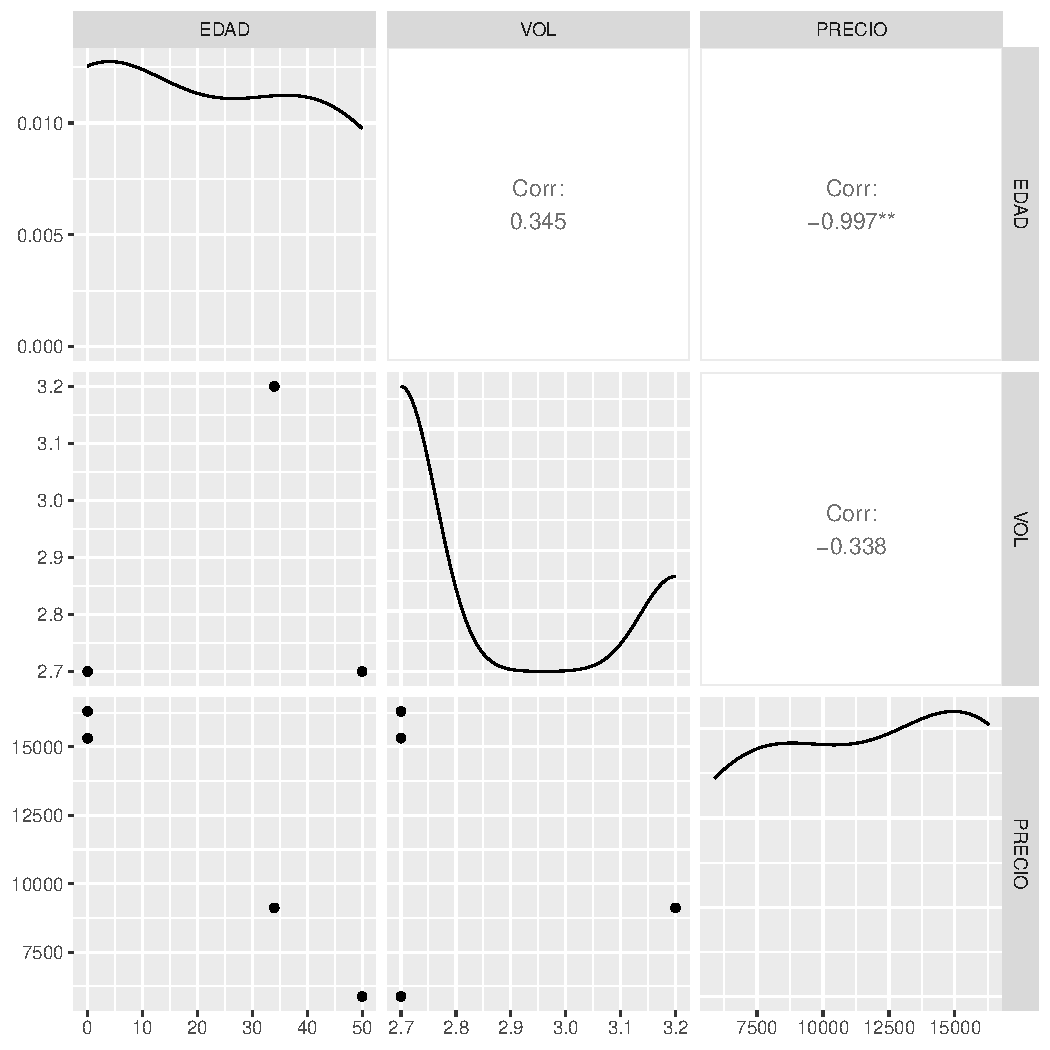
\includegraphics[width= 0.5 \linewidth, page=1]{../0.documentos/3_MERGED_MARKET/3_BOMBO_BATIDOR/r/Rplots.pdf}
    \end{minipage} 
    &
		Se tiene una correlación lineal negativa fuerte (el \(99.7\%\) de los datos lo corroboran),
		entre la Edad del Activo, y el Precio del Activo.
		\\ \hline 
  \end{tabular}
\end{center} 
% )))

\subsection{\centering --- Supuestos del Modelo de Regresión ---} % (((

Se realiza el análisis estadístico con un \(90\%\) de confianza. \\ 
Es decir, \(1- \alpha = 0.9\).

\subsubsection{--- Homocedasticidad ---} % (((
\begin{center}
  \begin{tabular}{|l|p{8cm}|}
    \cline{1-2}
    \multicolumn{2}{|c|}{Hipótesis}\\ \cline{1-2}
    \multicolumn{2}{|l|}{\(H_0:\) La varianza de los residuales es constante.} \\ 
    \multicolumn{2}{|l|}{\(H_a:\) La varianza de los residuales no es constante.} \\ \cline{1-2}
    Estadístico de Prueba & \(BP = 4\).\\ \cline{1-2} 
		Región de Rechazo de \(H_0\) & \((0, \alpha )\).\\ \cline{1-2} 
    Valor \(p\) & \(0.1353\).\\ \cline{1-2} 
    Conclusión & Se tiene que \(p> \alpha\). \newline 
		Por tanto no se rechaza \(H_0\). \newline 
		Es decir, la varianza no es constante. \\ \cline{1-2} 
  \end{tabular}
\end{center}
% )))

\subsubsection{--- Independencia ---} % (((
\begin{center}
  \begin{tabular}{|l|p{8cm}|}
    \cline{1-2}
    \multicolumn{2}{|c|}{Hipótesis}\\ \cline{1-2}
    \multicolumn{2}{|l|}{\(H_0:\) Los residuos son independientes.} \\ 
    \multicolumn{2}{|l|}{\(H_a:\) Los residuos no son indpendientes.} \\ \cline{1-2}
    Estadístico de Prueba & \(DW = 2.5\).\\ \cline{1-2} 
		Región de Rechazo de \(H_0\) & \((0, \alpha )\).\\ \cline{1-2} 
    Valor \(p\) & \(1\).\\ \cline{1-2} 
    Conclusión & Se tiene que \(p> \alpha\). \newline 
		Por tanto no se rechaza \(H_0\). \newline 
		Es decir, los residuos son independientes.\\ \cline{1-2} 
  \end{tabular}
\end{center}
% )))

\subsubsection{--- Normalidad ---} % (((
\begin{center}
  \begin{tabular}{|l|p{8cm}|}
    \cline{1-2}
    \multicolumn{2}{|c|}{Hipótesis}\\ \cline{1-2}
    \multicolumn{2}{|l|}{\(H_0:\) Los residuos siguen una distribución normal} \\ 
    \multicolumn{2}{|l|}{\(H_a:\) Los residuos no siguen una distribución normal.} \\ \cline{1-2}
    Estadístico de Prueba & \(W = 0.94466\).\\ \cline{1-2} 
		Región de Rechazo de \(H_0\) & \((0, \alpha )\).\\ \cline{1-2} 
    Valor \(p\) & \(0.683\).\\ \cline{1-2} 
    Conclusión & Se tiene que \(p> \alpha\). \newline 
		Por tanto no se rechaza \(H_0\). \newline 
		Es decir, los residuos siguen una distribución normal.\\ \cline{1-2} 
  \end{tabular}
\end{center}
% )))

% )))

\subsection{\centering Modelo de Regresión Estimado ---} % (((
\begin{align}
	Y & = &              370,099 & - 4,749 \cdot X_1           & + 3,022     \cdot X_2   \\[2mm]
	\mbox{Precio} & = &  370,099 & - 4,749 \cdot (\mbox{Edad}) & + 3,022     \cdot (\mbox{Volumen})
	\label{eq:3}
\end{align}
% )))

\subsection{\centering --- Tabla Anova ---} % (((
\begin{center}
  \begin{tabular}{|l|l|l|l|l|}
    \hline 
Fuentes de Variación  & Suma de Cuadrados & Grados de Libertad & Cuadrados Medios & F\\ \hline 
Regresión  &  42487120937          &  2     &  21243560469 & 77.42292 \\ \hline
Error      &    274383350          &  1     &    274383350 &  0.00000 \\ \hline
Totales    &  42761504287          &  3     &  21517943819 &  0.00000 \\ \hline
  \end{tabular}
\end{center} 
% )))

\subsection{\centering --- Prueba de Significancia del Modelo ---} % (((
Se comprueba la significancia del modelo con el estadístico \(F\) de la Tabla Anova.
\begin{center}
  \begin{tabular}{|l|p{6cm}|}
    \cline{1-2}
    \multicolumn{2}{|c|}{Hipótesis}\\ \cline{1-2}
    \multicolumn{2}{|l|}{\(H_0:\) El modelo no es significativo.} \\ 
    \multicolumn{2}{|l|}{\(H_a:\) El modelo es significativo.} \\ \cline{1-2}
    Estadístico de Prueba & \(77.42292\).\\ \cline{1-2} 
		Región de Rechazo de \(H_0\) & \((0, \alpha )\).\\ \cline{1-2} 
    Valor \(p\) & \(0.0801\).\\ \cline{1-2} 
    Conclusión & Se tiene que \(p<\alpha\). \newline 
		Por tanto se rechaza \(H_0\). \newline 
		Es decir, el modelo es significativo.\\ \cline{1-2} 
  \end{tabular}
\end{center} 
% )))

\subsection{\centering Estimación del Valor de Mercado aplicado al Activo.} % (((
Se obtiene el valor de mercado por medio de las características del activo y el modelo de regresión \eqref{eq:3}.
\begin{center}
  \begin{tabular}{|l|l|l|}
    \hline 
		Descripción   & Unidades  & Activo \\ \hline 
    Edad del activo    & Años      & 5      \\ \hline 
		Volumen  & \(m ^ 3\) & 2.5   \\ \hline 
		Precio del activo   & MXN       & \$292,292.9   \\ \hline 
  \end{tabular}
\end{center} 
% )))

% )))

\section{Compresor Horizontal Oil-Free.} % (((
Se realizó el enfoque de mercado que involucra a los siguientes activos.

\subsection{\centering --- Variables ---} % (((
\begin{center}
  \begin{tabular}{|l|l|l|}
    \hline 
    Variable & Descripción   & Unidades\\ \hline 
    Y:  & Precio del activo  & MXN \\ \hline 
    X1: & Edad del activo    & Años \\ \hline 
		X2: & Capacidad  & \(hp\) \\ \hline 
  \end{tabular}
\end{center} 
% )))

\subsection{\centering --- Mercado Usado ---} % (((
Se toma la siguiente muestra estadísticamente significativa. \\ 
La comprobación de este hecho se realiza a lo largo de las siguientes secciones.
\begin{center}
	\begin{tabular}{*{4}{|p{3cm}}|}
		\hline 
MARCA          & EDAD  & POT  & PRECIO\\ \hline
Ingresoll Rand & 0     & 10   & \$105,913.72\\ \hline
Carrollair     & 0     & 10   & \$126,021.06\\ \hline
GK-660-2/16    & 32    & 7    & \$26,196.00\\ \hline
MH11           & 21    & 15   & \$32,172.75\\ \hline
CV             & 51    & 5    & \$10,862.50\\ \hline
1WD74          & 18    & 10   & \$43,450.00\\ \hline
	\end{tabular}
\end{center}
% )))

\subsection{\centering --- Matriz de Dispersion ---} % (((
\begin{center}
  \begin{tabular}{|p{11cm}|p{5cm}|}
    \hline
    Gráfica & Interpretación. \\ \hline 
    \begin{minipage}{\textwidth}
    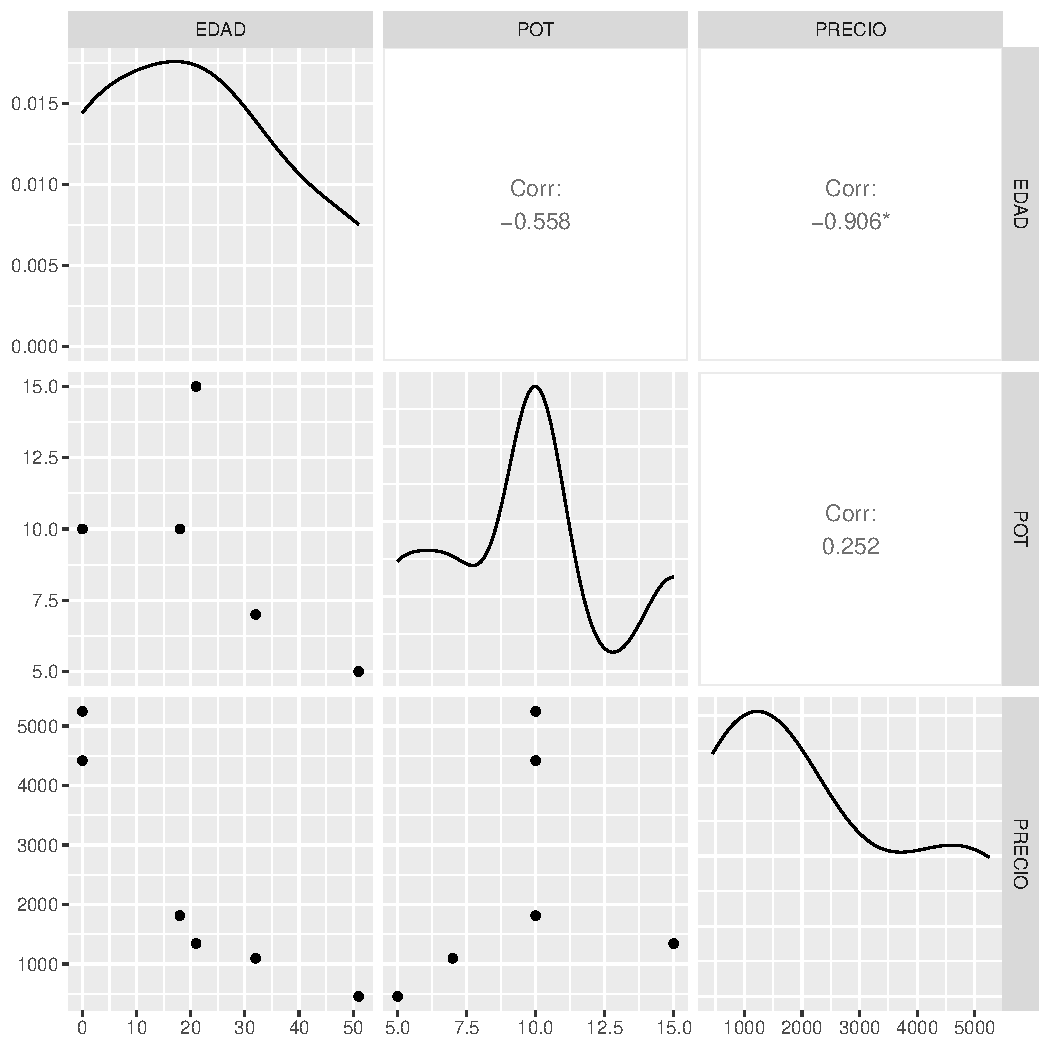
\includegraphics[width= 0.5 \linewidth, page=1]{../0.documentos/3_MERGED_MARKET/4_COMPRESOR_AIRE_OIL_FREE/r/Rplots.pdf}
    \end{minipage} 
    &
		Se tiene una correlación lineal negativa fuerte (el \(90.6\%\) de los datos lo corroboran),
		entre la Edad del Activo, y el Precio del Activo.
		\\ \hline 
  \end{tabular}
\end{center} 
% )))

\subsection{\centering --- Supuestos del Modelo de Regresión ---} % (((

Se realiza el análisis estadístico con un \(90\%\) de confianza. \\ 
Es decir, \(1- \alpha = 0.9\).

\subsubsection{--- Homocedasticidad ---} % (((
\begin{center}
  \begin{tabular}{|l|p{8cm}|}
    \cline{1-2}
    \multicolumn{2}{|c|}{Hipótesis}\\ \cline{1-2}
    \multicolumn{2}{|l|}{\(H_0:\) La varianza de los residuales es constante.} \\ 
    \multicolumn{2}{|l|}{\(H_a:\) La varianza de los residuales no es constante.} \\ \cline{1-2}
    Estadístico de Prueba & \(BP = 0.89468\).\\ \cline{1-2} 
		Región de Rechazo de \(H_0\) & \((0, \alpha )\).\\ \cline{1-2} 
    Valor \(p\) & \(0.6393\).\\ \cline{1-2} 
    Conclusión & Se tiene que \(p> \alpha\). \newline 
		Por tanto no se rechaza \(H_0\). \newline 
		Es decir, la varianza no es constante. \\ \cline{1-2} 
  \end{tabular}
\end{center}
% )))

\subsubsection{--- Independencia ---} % (((
\begin{center}
  \begin{tabular}{|l|p{8cm}|}
    \cline{1-2}
    \multicolumn{2}{|c|}{Hipótesis}\\ \cline{1-2}
    \multicolumn{2}{|l|}{\(H_0:\) Los residuos son independientes.} \\ 
    \multicolumn{2}{|l|}{\(H_a:\) Los residuos no son indpendientes.} \\ \cline{1-2}
    Estadístico de Prueba & \(DW = 2.6999\).\\ \cline{1-2} 
		Región de Rechazo de \(H_0\) & \((0, \alpha )\).\\ \cline{1-2} 
    Valor \(p\) & \(0.8643\).\\ \cline{1-2} 
    Conclusión & Se tiene que \(p> \alpha\). \newline 
		Por tanto no se rechaza \(H_0\). \newline 
		Es decir, los residuos son independientes.\\ \cline{1-2} 
  \end{tabular}
\end{center}
% )))

\subsubsection{--- Normalidad ---} % (((
\begin{center}
  \begin{tabular}{|l|p{8cm}|}
    \cline{1-2}
    \multicolumn{2}{|c|}{Hipótesis}\\ \cline{1-2}
    \multicolumn{2}{|l|}{\(H_0:\) Los residuos siguen una distribución normal} \\ 
    \multicolumn{2}{|l|}{\(H_a:\) Los residuos no siguen una distribución normal.} \\ \cline{1-2}
    Estadístico de Prueba & \(W = 0.94854\).\\ \cline{1-2} 
		Región de Rechazo de \(H_0\) & \((0, \alpha )\).\\ \cline{1-2} 
    Valor \(p\) & \(0.7285\).\\ \cline{1-2} 
    Conclusión & Se tiene que \(p> \alpha\). \newline 
		Por tanto no se rechaza \(H_0\). \newline 
		Es decir, los residuos siguen una distribución normal.\\ \cline{1-2} 
  \end{tabular}
\end{center}
% )))

% )))

\subsection{\centering Modelo de Regresión Estimado ---} % (((
\begin{align}
	Y & = &              160,408 & - 2,673 \cdot X_1           & - 5,118     \cdot X_2   \\[2mm]
	\mbox{Precio} & = &  160,408 & - 2,673 \cdot (\mbox{Edad}) & - 5,118     \cdot (\mbox{hp})
	\label{eq:4}
\end{align}
% )))

\subsection{\centering --- Tabla Anova ---} % (((
\begin{center}
  \begin{tabular}{|l|l|l|l|l|}
    \hline 
    Fuentes de Variación  & Suma de Cuadrados & Grados de Libertad & Cuadrados Medios & F\\ \hline 
Regresión  &  10087994715          &  2       & 5043997358 & 16.01483\\ \hline
Error      &    944873575          &  3       &  314957858 &  0.00000\\ \hline
Totales    &  11032868290          &  5       & 5358955216 &  0.00000\\ \hline
  \end{tabular}
\end{center} 
% )))

\subsection{\centering --- Prueba de Significancia del Modelo ---} % (((
Se comprueba la significancia del modelo con el estadístico \(F\) de la Tabla Anova.
\begin{center}
  \begin{tabular}{|l|p{6cm}|}
    \cline{1-2}
    \multicolumn{2}{|c|}{Hipótesis}\\ \cline{1-2}
    \multicolumn{2}{|l|}{\(H_0:\) El modelo no es significativo.} \\ 
    \multicolumn{2}{|l|}{\(H_a:\) El modelo es significativo.} \\ \cline{1-2}
    Estadístico de Prueba & \(16.01\).\\ \cline{1-2} 
		Región de Rechazo de \(H_0\) & \((0, \alpha )\).\\ \cline{1-2} 
    Valor \(p\) & \(0.02506\).\\ \cline{1-2} 
    Conclusión & Se tiene que \(p<\alpha\). \newline 
		Por tanto se rechaza \(H_0\). \newline 
		Es decir, el modelo es significativo.\\ \cline{1-2} 
  \end{tabular}
\end{center} 
% )))

\subsection{\centering Estimación del Valor de Mercado aplicado al Activo.} % (((
Se obtiene el valor de mercado por medio de las características del activo y el modelo de regresión \eqref{eq:4}.
\begin{center}
  \begin{tabular}{|l|l|l|}
    \hline 
		Descripción   & Unidades  & Activo \\ \hline 
    Edad del activo    & Años      & 5      \\ \hline 
		Toneladas de cap.  & \(hp\) & 10   \\ \hline 
		Precio del activo   & MXN       & \$74,836.82   \\ \hline 
  \end{tabular}
\end{center} 
% )))

% )))

\section{Secador de Aire, Tipo Refrigerado.} % (((
Se realizó el enfoque de mercado que involucra a los siguientes activos.

\subsection{\centering --- Variables ---} % (((
\begin{center}
  \begin{tabular}{|l|l|l|}
    \hline 
    Variable & Descripción   & Unidades\\ \hline 
    Y:  & Precio del activo  & MXN \\ \hline 
    X1: & Edad del activo    & Años \\ \hline 
		X2: & Capacidad & \(hp\) \\ \hline 
  \end{tabular}
\end{center} 
% )))

\subsection{\centering --- Mercado Usado ---} % (((
Se toma la siguiente muestra estadísticamente significativa. \\ 
La comprobación de este hecho se realiza a lo largo de las siguientes secciones.
\begin{center}
	\begin{tabular}{*{4}{|p{3cm}}|}
		\hline 
MARCA          & EDAD  & CAP  & PRECIO\\ \hline
Speedaire      & 0     & 35   & 104750.90\\ \hline
Hankison       & 0     & 25   & 54461.60\\ \hline
Ingersoll Rand & 0     & 15   & 151014.60\\ \hline
Atlas Copco    & 11    & 14   & 31224.75\\ \hline
Beko           & 4     & 50   & 27650.00\\ \hline
Kaeser         & 11    & 20   & 18555.50\\ \hline
Atlas Copco    & 3     & 63   & 28379.00\\ \hline
Atlas Copco    & 18    & 32   & 15701.25\\ \hline
	\end{tabular}
\end{center}
% )))

\subsection{\centering --- Matriz de Dispersion ---} % (((
\begin{center}
  \begin{tabular}{|p{11cm}|p{5cm}|}
    \hline
    Gráfica & Interpretación. \\ \hline 
    \begin{minipage}{\textwidth}
    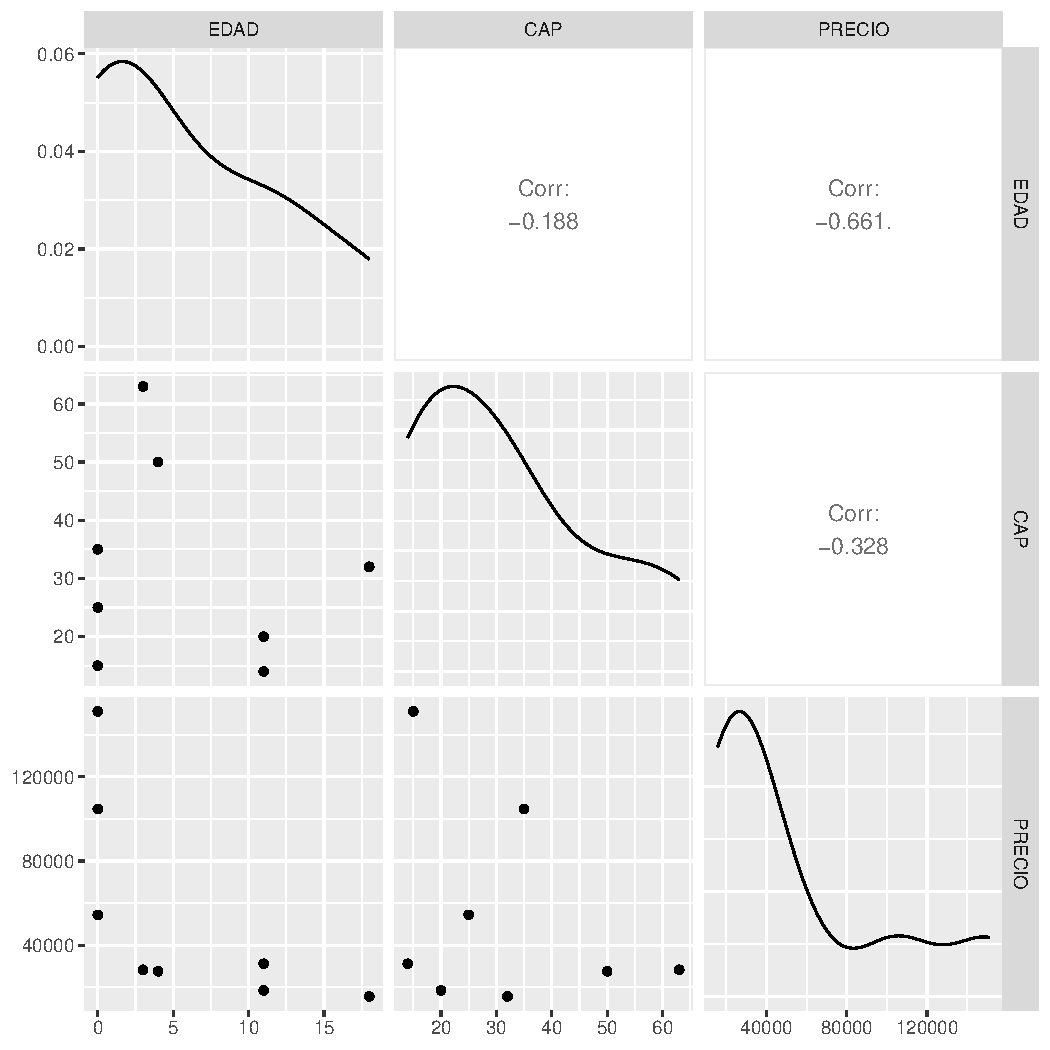
\includegraphics[width= 0.5 \linewidth, page=1]{../0.documentos/3_MERGED_MARKET/5_SECADOR_AIRE/r/Rplots.pdf}
    \end{minipage} 
    &
		Hay una correlación lineal débil (el \(66.1\%\) de los datos lo confirman),
		entre la Edad y el Precio del activo.
		\\ \hline 
  \end{tabular}
\end{center} 
% )))

\subsection{\centering --- Supuestos del Modelo de Regresión ---} % (((

Se realiza el análisis estadístico con un \(90\%\) de confianza. \\ 
Es decir, \(1- \alpha = 0.9\).

\subsubsection{--- Homocedasticidad ---} % (((
\begin{center}
  \begin{tabular}{|l|p{8cm}|}
    \cline{1-2}
    \multicolumn{2}{|c|}{Hipótesis}\\ \cline{1-2}
    \multicolumn{2}{|l|}{\(H_0:\) La varianza de los residuales es constante.} \\ 
    \multicolumn{2}{|l|}{\(H_a:\) La varianza de los residuales no es constante.} \\ \cline{1-2}
    Estadístico de Prueba & \(BP = 4.4606\).\\ \cline{1-2} 
		Región de Rechazo de \(H_0\) & \((0, \alpha )\).\\ \cline{1-2} 
    Valor \(p\) & \(0.1075\).\\ \cline{1-2} 
    Conclusión & Se tiene que \(p> \alpha\). \newline 
		Por tanto no se rechaza \(H_0\). \newline 
		Es decir, la varianza no es constante. \\ \cline{1-2} 
  \end{tabular}
\end{center}
% )))

\subsubsection{--- Independencia ---} % (((
\begin{center}
  \begin{tabular}{|l|p{8cm}|}
    \cline{1-2}
    \multicolumn{2}{|c|}{Hipótesis}\\ \cline{1-2}
    \multicolumn{2}{|l|}{\(H_0:\) Los residuos son independientes.} \\ 
    \multicolumn{2}{|l|}{\(H_a:\) Los residuos no son indpendientes.} \\ \cline{1-2}
    Estadístico de Prueba & \(DW = 2.7842\).\\ \cline{1-2} 
		Región de Rechazo de \(H_0\) & \((0, \alpha )\).\\ \cline{1-2} 
    Valor \(p\) & \(0.9005\).\\ \cline{1-2} 
    Conclusión & Se tiene que \(p> \alpha\). \newline 
		Por tanto no se rechaza \(H_0\). \newline 
		Es decir, los residuos son independientes.\\ \cline{1-2} 
  \end{tabular}
\end{center}
% )))

\subsubsection{--- Normalidad ---} % (((
\begin{center}
  \begin{tabular}{|l|p{8cm}|}
    \cline{1-2}
    \multicolumn{2}{|c|}{Hipótesis}\\ \cline{1-2}
    \multicolumn{2}{|l|}{\(H_0:\) Los residuos siguen una distribución normal} \\ 
    \multicolumn{2}{|l|}{\(H_a:\) Los residuos no siguen una distribución normal.} \\ \cline{1-2}
    Estadístico de Prueba & \(W = 0.95507\).\\ \cline{1-2} 
		Región de Rechazo de \(H_0\) & \((0, \alpha )\).\\ \cline{1-2} 
    Valor \(p\) & \(0.7621\).\\ \cline{1-2} 
    Conclusión & Se tiene que \(p> \alpha\). \newline 
		Por tanto no se rechaza \(H_0\). \newline 
		Es decir, los residuos siguen una distribución normal.\\ \cline{1-2} 
  \end{tabular}
\end{center}
% )))

% )))

\subsection{\centering Modelo de Regresión Estimado ---} % (((
\begin{align}
	Y & = &              127,764 & - 5,439 \cdot X_1           & - 1,318     \cdot X_2   \\[2mm]
	\mbox{Precio} & = &  127,764 & - 5,439 \cdot (\mbox{Edad}) & - 1,318     \cdot (\mbox{hp})
	\label{eq:5}
\end{align}
% )))

\subsection{\centering --- Tabla Anova ---} % (((
\begin{center}
  \begin{tabular}{|l|l|l|l|l|}
    \hline 
    Fuentes de Variación  & Suma de Cuadrados & Grados de Libertad & Cuadrados Medios & F\\ \hline 
Regresión  & 10763470574          &  2       & 5381735287 & 4.62603\\ \hline
Error      &  5816797343          &  5       & 1163359469 & 0.00000\\ \hline
Totales    & 16580267917          &  7       & 6545094756 & 0.00000\\ \hline
  \end{tabular}
\end{center} 
% )))

\subsection{\centering --- Prueba de Significancia del Modelo ---} % (((
Se comprueba la significancia del modelo con el estadístico \(F\) de la Tabla Anova.
\begin{center}
  \begin{tabular}{|l|p{6cm}|}
    \cline{1-2}
    \multicolumn{2}{|c|}{Hipótesis}\\ \cline{1-2}
    \multicolumn{2}{|l|}{\(H_0:\) El modelo no es significativo.} \\ 
    \multicolumn{2}{|l|}{\(H_a:\) El modelo es significativo.} \\ \cline{1-2}
    Estadístico de Prueba & \(4.626\).\\ \cline{1-2} 
		Región de Rechazo de \(H_0\) & \((0, \alpha )\).\\ \cline{1-2} 
    Valor \(p\) & \(0.0729\).\\ \cline{1-2} 
    Conclusión & Se tiene que \(p<\alpha\). \newline 
		Por tanto se rechaza \(H_0\). \newline 
		Es decir, el modelo es significativo.\\ \cline{1-2} 
  \end{tabular}
\end{center} 
% )))

\subsection{\centering Estimación del Valor de Mercado aplicado al Activo.} % (((
Se obtiene el valor de mercado por medio de las características del activo y el modelo de regresión \eqref{eq:5}.
\begin{center}
  \begin{tabular}{|l|l|l|}
    \hline 
		Descripción   & Unidades  & Activo \\ \hline 
    Edad del activo    & Años      & 2      \\ \hline 
		Capacidad  & \(hp\) & 35   \\ \hline 
		Precio del activo   & MXN       & \$59,786.41   \\ \hline 
  \end{tabular}
\end{center} 
% )))
% )))

\section{Compresor Tipo Tornillo.} % (((
Se realizó el enfoque de mercado que involucra a los siguientes activos.

\subsection{\centering --- Variables ---} % (((
\begin{center}
  \begin{tabular}{|l|l|l|}
    \hline 
    Variable & Descripción   & Unidades\\ \hline 
    Y:  & Precio del activo  & MXN \\ \hline 
    X1: & Edad del activo    & Años \\ \hline 
		X2: & Potencia  & \(hp\) \\ \hline 
  \end{tabular}
\end{center} 
% )))

\subsection{\centering --- Mercado Usado ---} % (((
Se toma la siguiente muestra estadísticamente significativa. \\ 
La comprobación de este hecho se realiza a lo largo de las siguientes secciones.
\begin{center}
	\begin{tabular}{*{4}{|p{2cm}}|}
		\hline 
MARCA          &  EDAD  & POT  & PRECIO\\ \hline
EVANS          &  0     & 75   & 570862.00\\ \hline
Ingresoll Rand &  13    & 100  & 237785.00\\ \hline
Ingresoll Rand &  15    & 50   & 219352.00\\ \hline
ALMIG          &  15    & 100  & 225503.90\\ \hline
	\end{tabular}
\end{center}
% )))

\subsection{\centering --- Matriz de Dispersion ---} % (((
\begin{center}
  \begin{tabular}{|p{11cm}|p{5cm}|}
    \hline
    Gráfica & Interpretación. \\ \hline 
    \begin{minipage}{\textwidth}
    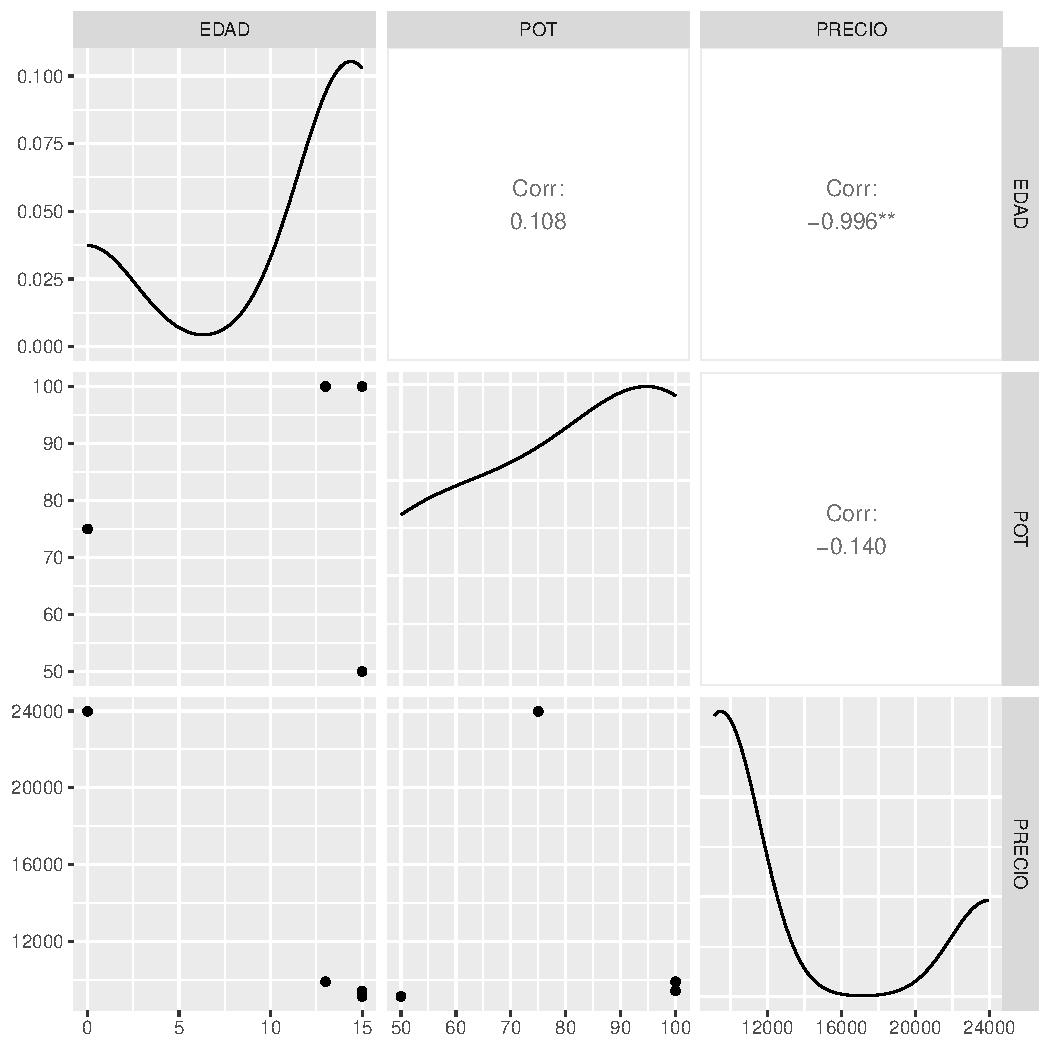
\includegraphics[width= 0.5 \linewidth, page=1]{../0.documentos/3_MERGED_MARKET/6_COMPRESOR_TIPO_TORNILLO/r/Rplots.pdf}
    \end{minipage} 
    &
		Se tiene una correlación lineal negativa fuerte (el \(99.6\%\) de los datos lo corroboran),
		entre la Edad del Activo, y el Precio del Activo.
		\\ \hline 
  \end{tabular}
\end{center} 
% )))

\subsection{\centering --- Supuestos del Modelo de Regresión ---} % (((

Se realiza el análisis estadístico con un \(90\%\) de confianza. \\ 
Es decir, \(1- \alpha = 0.9\).

\subsubsection{--- Homocedasticidad ---} % (((
\begin{center}
  \begin{tabular}{|l|p{8cm}|}
    \cline{1-2}
    \multicolumn{2}{|c|}{Hipótesis}\\ \cline{1-2}
    \multicolumn{2}{|l|}{\(H_0:\) La varianza de los residuales es constante.} \\ 
    \multicolumn{2}{|l|}{\(H_a:\) La varianza de los residuales no es constante.} \\ \cline{1-2}
    Estadístico de Prueba & \(BP = 3.9163\).\\ \cline{1-2} 
		Región de Rechazo de \(H_0\) & \((0, \alpha )\).\\ \cline{1-2} 
    Valor \(p\) & \(0.1411\).\\ \cline{1-2} 
    Conclusión & Se tiene que \(p> \alpha\). \newline 
		Por tanto no se rechaza \(H_0\). \newline 
		Es decir, la varianza no es constante. \\ \cline{1-2} 
  \end{tabular}
\end{center}
% )))

\subsubsection{--- Independencia ---} % (((
\begin{center}
  \begin{tabular}{|l|p{8cm}|}
    \cline{1-2}
    \multicolumn{2}{|c|}{Hipótesis}\\ \cline{1-2}
    \multicolumn{2}{|l|}{\(H_0:\) Los residuos son independientes.} \\ 
    \multicolumn{2}{|l|}{\(H_a:\) Los residuos no son indpendientes.} \\ \cline{1-2}
    Estadístico de Prueba & \(DW = 1.6667\).\\ \cline{1-2} 
		Región de Rechazo de \(H_0\) & \((0, \alpha )\).\\ \cline{1-2} 
    Valor \(p\) & \(1\).\\ \cline{1-2} 
    Conclusión & Se tiene que \(p> \alpha\). \newline 
		Por tanto no se rechaza \(H_0\). \newline 
		Es decir, los residuos son independientes.\\ \cline{1-2} 
  \end{tabular}
\end{center}
% )))

\subsubsection{--- Normalidad ---} % (((
\begin{center}
  \begin{tabular}{|l|p{8cm}|}
    \cline{1-2}
    \multicolumn{2}{|c|}{Hipótesis}\\ \cline{1-2}
    \multicolumn{2}{|l|}{\(H_0:\) Los residuos siguen una distribución normal} \\ 
    \multicolumn{2}{|l|}{\(H_a:\) Los residuos no siguen una distribución normal.} \\ \cline{1-2}
    Estadístico de Prueba & \(W = 0.97975\).\\ \cline{1-2} 
		Región de Rechazo de \(H_0\) & \((0, \alpha )\).\\ \cline{1-2} 
    Valor \(p\) & \(0.9005\).\\ \cline{1-2} 
    Conclusión & Se tiene que \(p> \alpha\). \newline 
		Por tanto no se rechaza \(H_0\). \newline 
		Es decir, los residuos siguen una distribución normal.\\ \cline{1-2} 
  \end{tabular}
\end{center}
% )))

% )))

\subsection{\centering Modelo de Regresión Estimado ---} % (((
\begin{align}
	Y & = &              586,304 & - 23,590 \cdot X_1           & - 238     \cdot X_2   \\[2mm]
	\mbox{Precio} & = &  586,304 & - 23,590 \cdot (\mbox{Edad}) & - 238     \cdot (\mbox{hp})
	\label{eq:6}
\end{align}
% )))

\subsection{\centering --- Tabla Anova ---} % (((
\begin{center}
  \begin{tabular}{|l|l|l|l|l|}
    \hline 
    Fuentes de Variación  & Suma de Cuadrados & Grados de Libertad & Cuadrados Medios & F\\ \hline 
Regresión  &  87958129225          &  2      & 43979064612 & 71.2871\\ \hline
Error      &    616928786          &  1      &   616928786 &  0.0000\\ \hline
Totales    &  88575058011          &  3      & 44595993399 &  0.0000\\ \hline
  \end{tabular}
\end{center} 
% )))

\subsection{\centering --- Prueba de Significancia del Modelo ---} % (((
Se comprueba la significancia del modelo con el estadístico \(F\) de la Tabla Anova.
\begin{center}
  \begin{tabular}{|l|p{6cm}|}
    \cline{1-2}
    \multicolumn{2}{|c|}{Hipótesis}\\ \cline{1-2}
    \multicolumn{2}{|l|}{\(H_0:\) El modelo no es significativo.} \\ 
    \multicolumn{2}{|l|}{\(H_a:\) El modelo es significativo.} \\ \cline{1-2}
    Estadístico de Prueba & \(71.29\).\\ \cline{1-2} 
		Región de Rechazo de \(H_0\) & \((0, \alpha )\).\\ \cline{1-2} 
    Valor \(p\) & \(0.08346\).\\ \cline{1-2} 
    Conclusión & Se tiene que \(p<\alpha\). \newline 
		Por tanto se rechaza \(H_0\). \newline 
		Es decir, el modelo es significativo.\\ \cline{1-2} 
  \end{tabular}
\end{center} 
% )))

\subsection{\centering Estimación del Valor de Mercado aplicado al Activo.} % (((
Se obtiene el valor de mercado por medio de las características del activo y el modelo de regresión \eqref{eq:6}.
\begin{center}
  \begin{tabular}{|l|l|l|}
    \hline 
		Descripción   & Unidades  & Activo \\ \hline 
    Edad del activo    & Años      & 2      \\ \hline 
		Capacidad  & \(hp\) & 75   \\ \hline 
		Precio del activo   & MXN       & \$482,536.1   \\ \hline 
  \end{tabular}
\end{center} 
% )))

% )))

% )))
